\documentclass[10pt, table, dvipsnames,xcdraw]{beamer}
\usetheme[progressbar=frametitle]{metropolis}
\usepackage{appendixnumberbeamer}
\usetikzlibrary{arrows.meta, positioning, quotes}
\usepackage[shortlabels]{enumitem}
\usepackage{xcolor}
\usepackage{mathtools}
\usepackage{dsfont}


\usepackage{cancel}

\newcommand\hcancel[2][black]{\setbox0=\hbox{$#2$}%
\rlap{\raisebox{.45\ht0}{\textcolor{#1}{\rule{\wd0}{1pt}}}}#2} 


\usepackage{booktabs}
\usepackage[scale=2]{ccicons}

\usepackage{pgfplots}
\usepgfplotslibrary{dateplot}

\usepackage{xspace}
\newcommand{\themename}{\textbf{\textsc{metropolis}}\xspace}
\newcommand{\cb}{\cellcolor{blue!25}}


% Notation:
\newcommand{\cT}{\ensuremath{\mathcal{T}}}
\newcommand{\cD}{\ensuremath{\mathcal{D}}}
\newcommand{\cX}{\ensuremath{\mathcal{X}}}
\newcommand{\cY}{\ensuremath{\mathcal{Y}}}
\newcommand{\cZ}{\ensuremath{\mathcal{Z}}}
\newcommand{\cH}{\ensuremath{\mathcal{H}}}
\newcommand{\cG}{\ensuremath{\mathcal{G}}}

\newcommand{\bR}{\ensuremath{\mathbb{R}}}
\newcommand{\bN}{\ensuremath{\mathbb{N}}}
\newcommand{\bP}{\ensuremath{\mathbb{P}}}
\newcommand{\bT}{\ensuremath{\mathbb{T}}}
\newcommand{\bL}{\ensuremath{\mathbb{L}}}

\newcommand{\bfX}{\ensuremath{\mathbf{X}}}
\newcommand{\bfY}{\ensuremath{\mathbf{Y}}}
\newcommand{\bfy}{\ensuremath{\mathbf{y}}}

\def\layersep{2.5cm}

% Tikz seys
\tikzset{cross/.style={cross out, draw, 
         minimum size=2*(#1-\pgflinewidth), 
         inner sep=0pt, outer sep=0pt}}

\title{Machine Learning I}
\subtitle{Lecture 13: Decision Trees and Support Vector Machines}
% \date{\today}
\date{}
\author{Nathaniel Bade}
\institute{Northeastern University Department of Mathematics}
% \titlegraphic{\hfill\includegraphics[height=1.5cm]{logo.pdf}}

\begin{document}

\maketitle

\begin{frame}{Table of contents}
  \setbeamertemplate{section in toc}[sections numbered]
  \tableofcontents[hideallsubsections]
\end{frame}


%%%%%%%%%%%%%% Slidshow Start %%%%%%%%%%%%%% 



\section{Decision Trees}

\begin{frame}[fragile]{Decision Tree Example: Titanic Dataset}
\begin{table}[]
\begin{tabular}{|l|l|l|l|l|l|l|l|}
\hline
\rowcolor[HTML]{656565} 
{\color[HTML]{EFEFEF} Pclass} & {\color[HTML]{EFEFEF} Name} & \multicolumn{1}{c|}{\cellcolor[HTML]{656565}{\color[HTML]{EFEFEF} Sex}} & {\color[HTML]{EFEFEF} Age} & {\color[HTML]{EFEFEF} SibSp} & {\color[HTML]{EFEFEF} Parch}  & {\color[HTML]{FFFFFF} Emb} & {\color[HTML]{FFFFFF} Sur} \\ \hline
3                             & Kelly, James            & m                                                                       & 34.5                       & 0                            & 0                                                & Q    & 0                           \\ \hline
3                             & Connolly, Kate        & f                                                                       & 30.0                       & 0                            & 1                                                 & S    & 0                           \\ \hline
2                             & McFerson, Jack        & m                                                                       & 53.0                       & 0                            & 1                                                 & S    & 1                           \\ \hline
\end{tabular}
\end{table}
  \vfill
\begin{minipage}[t][0.5\textheight][t]{\textwidth}
In the titanic dataset, we try to predict survivors (\textbf{Sur}) based on (\textbf{Age}), ticket class (\textbf{Pclass}), \textbf{sex}, number of siblings/spouse present (\textbf{SibSp}), parents or children (\textbf{Parch}) and embarkment port (\textbf{Emb}). \pause \newline 

Tree based methods provide clear explanations of their fitting methodology. A binary decision tree classifies the data based on partitioning each feature into two sets at each step. 
\end{minipage}
\end{frame}



\begin{frame}[fragile]{Decision Tree Example: Titanic Dataset}
  \begin{minipage}[t][0.6\textheight][t]{\textwidth}
	\centering \includegraphics[height=0.6\textheight]{L13Titanic1.png} 
  \end{minipage}
  \vfill
\begin{minipage}[t][0.4\textheight][t]{\textwidth}
\begin{table}[]
\begin{tabular}{|l|l|l|l|l|l|l|l|}
\hline
\rowcolor[HTML]{656565} 
{\color[HTML]{EFEFEF} Pclass} & {\color[HTML]{EFEFEF} Name} & \multicolumn{1}{c|}{\cellcolor[HTML]{656565}{\color[HTML]{EFEFEF} Sex}} & {\color[HTML]{EFEFEF} Age} & {\color[HTML]{EFEFEF} SibSp} & {\color[HTML]{EFEFEF} Parch}  & {\color[HTML]{FFFFFF} Emb} & {\color[HTML]{FFFFFF} Sur} \\ \hline
3                             & Kelly, James            & m                                                                       & 34.5                       & 0                            & 0                                                & Q    & 0                           \\ \hline
3                             & Connolly, Kate        & f                                                                       & 30.0                       & 0                            & 1                                                 & S    & 0                           \\ \hline
2                             & McFerson, Jack        & m                                                                       & 53.0                       & 0                            & 1                                                 & S    & 1                           \\ \hline
\end{tabular}
\end{table}
\end{minipage}
\end{frame}




\begin{frame}[fragile]{Decision Tree Example: Titanic Dataset}
  \begin{minipage}[t][0.6\textheight][t]{\textwidth}
	\centering \includegraphics[height=0.6\textheight]{L13Titanic1.png} 
  \end{minipage}
  \vfill
\begin{minipage}[t][0.4\textheight][t]{\textwidth}
Each node gives the proportion of people at that node that survived as a decimal, and the percent of to total population that node accounts for. \pause The first node says overall there is a .38  chance of surviving. 
\end{minipage}
\end{frame}




\begin{frame}[fragile]{Decision Tree Example: Titanic Dataset}
  \begin{minipage}[t][0.6\textheight][t]{\textwidth}
	\centering \includegraphics[height=0.6\textheight]{L13Titanic1.png} 
  \end{minipage}
  \vfill
\begin{minipage}[t][0.4\textheight][t]{\textwidth}
The first splitting tells us that there is a 65\% of being male, and males had .19 chance of survival, while there is a 35\% chance of being female and females have a .74 chance of surviving. \pause

Then, on the right branch, we see that for females not of third class, the survival rate goes up to .95, but for third class woman it was merely .5.
\end{minipage}
\end{frame}


\begin{frame}[fragile]{Decision Tree Example: Titanic Dataset}
  \begin{minipage}[t][0.6\textheight][t]{\textwidth}
	\centering \includegraphics[height=0.6\textheight]{L13Titanic1.png} 
  \end{minipage}
  \vfill
\begin{minipage}[t][0.4\textheight][t]{\textwidth}
A decision tree gives us a clear organization of the linear choices being made to classify the data, but it comes at a cost: decision trees have a high potential to over fit, especially to sparse noisy data. Therefore we need to understand what the algorithm is doing and what kind of control we have over it. 
\end{minipage}
\end{frame}



\begin{frame}[fragile]{Splitting on Features}
We will describe the CART (Classification And Regression Tree) method of decision tree fitting. The CART model fits a decision tree by recursive splitting along axis aligned dimensions. That is, it splits the data into two region along one feature and models the response by taking the mean label (or probability of each label for categorical data) in each region. \pause We choose the variable and split point to achieve the best fit. \pause\newline

Then, one or both of the regions is split again, and this continues until a stopping rule is applied. CART employees a greedy algorithm, simply selecting the beat feature to split on at each step. 
\end{frame}


\begin{frame}[fragile]{Splitting on Features}
  \begin{minipage}[t][0.5\textheight][t]{\textwidth}
	\centering \includegraphics[width=\textwidth]{L13Splitting2.png} 
  \end{minipage}
  \vfill
\begin{minipage}[t][0.5\textheight][t]{\textwidth}
For example, on two features $X_1$ and $X_2$, we can actually visualize the splitting. For each region above, the probability of each label in each region is given the by the mean label expression in that region. \pause The model is 
$$
\hat{f}(X)= \sum_{m=1}^5 c_m  \mathds{1}_{R_m}(X),.
$$
\end{minipage}
\end{frame}



\begin{frame}[fragile]{Fitting Regression Trees}
Let's now turn to fitting a regression tree to a binary labeling:\newline

Given training data $(x_i, y_i)$ with $p$ features $X_1,\ldots, X_p$, let us choose the loss function to be MSE and attempt to fit
$$
\hat{f}(X)= \sum_{m=1}^M c_m  \mathds{1}_{R_m}(X)\,.
$$ \pause 

We pick $c_m = \text{mean}(y_i|x_i\in R_m)$ to be the mean $y_i$ in the region. \pause At the first step, splitting $\mathcal{X}$ to minimize loss is the same as finding $R_1(j,s) = \{X|X_j\leq s\}$ and $R_2(j,s)=\{X|X_j>s\}$ such that 
$$
\min_{j,s}\left[ \min_{c_1} \sum_{x_i\in R_1(j,s)} (y_i-c_1)^2 + \min_{c_2} \sum_{x_i\in R_2(j,s)} (y_i-c_2)^2\right]\,.
$$\pause 
For any $(j,s)$, the inner part is minimized by $\hat c_k = \text{mean}(y_i|x_i\in R_k(j,s))$. Fitting the tree can be done by a series of $mj$ 1-variable regressions.
\end{frame}


\begin{frame}[fragile]{Bias-Variance Trees}
  \begin{minipage}[t][0.5\textheight][t]{\textwidth}
	\centering \includegraphics[height=.5\textheight]{L13LargeTree.png} 
  \end{minipage}
  \vfill
\begin{minipage}[t][0.5\textheight][t]{\textwidth}
Clearly, if we grow the tree large enough we will over-fit by effectively cutting $\cX$ into $N$ regions, each one containing a single data point. \pause In fact, a bit of thought shows that with a large enough tree we could fit any dataset with distinct points as so we are in danger of massive overfitting. Note, that a general tree with $k$ levels will have $2^{k-1}$ terminal nodes. 
\end{minipage}
\end{frame}




\begin{frame}[fragile]{Bias-Variance Trees}
  \begin{minipage}[t][0.5\textheight][t]{\textwidth}
	\centering \includegraphics[height=.5\textheight]{L13LargeTree.png} 
  \end{minipage}
  \vfill
\begin{minipage}[t][0.5\textheight][t]{\textwidth}
On the other hand, sometimes good splits are hidden beneath poor ones. \textbf{Pruning}, rather than stopping growth, lets us find these without increasing variance too much. The idea behind pruning is to grow the tree past the point where the validation curve is diverging from the training error curve, and then to cut the tree.
\end{minipage}
\end{frame}





\begin{frame}[fragile]{Pruning Regression Trees}

In \textbf{cost-complexity pruning}, we want to minimize the error in each region while also penalizing the tree for growing too large. Let $m$ be index the terminal nodes in $T$ and the regions $R_m$. Let $N_m$ be the number of training points in each $R_m$ and let $\hat{c}_m$ be the average label in $R_m$. \pause Let
\[
Q_m(T) = \sum_{x_i\in R_m}(y_i-\hat{c}_m)^2\
\] 
be the un-normalized error in $R$. \pause Then the \textbf{cost-complexity criteria} is that we minimize
$$
C_\alpha(T) = \sum_{m=1}^{|T|} Q_m(T) + \alpha|T|\,,
$$
where $|T|$ is the number of terminal nodes remaining in $T$. \pause
\end{frame}





\begin{frame}[fragile]{Bias-Variance Trees}
  \begin{minipage}[t][0.5\textheight][t]{\textwidth}
	\centering \includegraphics[height=.5\textheight]{L13Titanic1.png} 
  \end{minipage}
  \vfill
\begin{minipage}[t][0.5\textheight][t]{\textwidth}
For example, lets compare our tree grown for the titanic data
\end{minipage}
\end{frame}



\begin{frame}[fragile]{Bias-Variance Trees}
  \begin{minipage}[t][0.5\textheight][t]{\textwidth}
	\centering \includegraphics[height=.5\textheight]{L13Pruning.png} 
  \end{minipage}
  \vfill
\begin{minipage}[t][0.5\textheight][t]{\textwidth}
For example, lets compare our tree grown for the titanic data, with the pruning of the much larger tree found before. We have found a new nontrivial split in the data. 
\end{minipage}
\end{frame}



\begin{frame}[fragile]{Classification}
To perform classification with a random tree, we need only specify the target error and the splitting criteria. Instead of trying to minimize $\frac{1}{N_m}Q_m$, for each region $R_m$, let
$$
\hat{p}_{mk} = \frac{1}{N_m}\sum_{x_i\in R_m}\mathds{1}(y_i = k)
$$ 
be the sample probability of label $k$ in region $m$. \pause Letting $k(m) = \text{argmax}_k(p_{mk})$ be the most probable label for node $m$, {node impurity} can be measured by
\begin{flalign*}
\text{Misclass. Error:}&& 1 - \hat{p}_{mk(m)} = \frac{1}{N_m}&\sum_{i\in R_m}\mathds{1}(y_i \neq k(m))&&
\\
\text{Gini Index:}&& \sum_{k\neq k'} \hat{p}_{mk} \hat{p}_{mk'} = &\sum_{k=1}^K  \hat{p}_{mk}(1-\hat{p}_{mk})&&
\\
\text{Cross-entropy:}&& &\sum_{k=1}^K\hat{p}_{mk}\log \hat{p}_{mk}&&
\end{flalign*}
\end{frame}




\begin{frame}[fragile]{Classification}
Why use an error besides the average misclassification error? While misclassification may be the most sensible error for a single node when we average the misclassification error across nodes we may lose a significant ``good'' split just because it doesn't contain very many elements. Lets look at an example. 
\begin{flalign*}
\text{Misclass. Error:}&& 1 - \hat{p}_{mk(m)} = \frac{1}{N_m}&\sum_{i\in R_m}\mathds{1}(y_i = k(m))&&
\\
\text{Gini Index:}&& \sum_{k\neq k'} \hat{p}_{mk} \hat{p}_{mk'} = &\sum_{k=1}^K  \hat{p}_{mk}(1-\hat{p}_{mk})&&
\\
\text{Cross-entropy:}&& &\sum_{k=1}^K\hat{p}_{mk}\log \hat{p}_{mk}&&
\end{flalign*}
\end{frame}



\begin{frame}[fragile]{Splitting Loss Functions: Misclassification}
For example, for two classes $L$ and $R$ with 40 observations in each class, say a split creates nodes $N_1 = (30,10)$ and $N_2 = (10,30)$ while another node creates $N_3 = (20,40)$, $N_4 = (20,0)$. \pause Then
\begin{align*}
\hat{p}_{1L} & = .75 & \hat{p}_{2L} & = .25 & \hat{p}_{3L} & = .333 & \hat{p}_{4L} & = 1 
\\
\hat{p}_{1R} & = .25 & \hat{p}_{2R} & = .75 & \hat{p}_{3R} & = .666 & \hat{p}_{4R} & = 0
\end{align*}\pause
Then, the misclassification error at splitting 1 is
\begin{flalign*}
\boxed{\text{Split 1:}} && \frac{N_1}{N}(1-\hat{p}_{1k(1)} )  + \frac{N_2}{N}(1-\hat{p}_{2k(2)} )   = \frac{40}{80}.25 + \frac{40}{80}.25 = .25\,,
\end{flalign*}\pause 
and at splitting 2, 
\begin{flalign*}
\boxed{\text{Split 2:}} &&  \frac{N_3}{N}(1-\hat{p}_{3k(3)} )  + \frac{N_4}{N}(1-\hat{p}_{4k(4)} ) =   \frac{60}{80}.333 + \frac{20}{80} \cdot 0 = .25\,.
\end{flalign*}

\end{frame}


\begin{frame}[fragile]{Splitting Loss Functions: Gini Index}
For example, for two classes $L$ and $R$ with 40 observations in each class, say a split creates nodes $N_1 = (30,10)$ and $N_2 = (10,30)$ while another node creates $N_3 = (20,40)$, $N_4 = (20,0)$. Then
\begin{align*}
\hat{p}_{1L} & = .75 & \hat{p}_{2L} & = .25 & \hat{p}_{3L} & = .333 & \hat{p}_{4L} & = 1 
\\
\hat{p}_{1R} & = .25 & \hat{p}_{2R} & = .75 & \hat{p}_{3R} & = .666 & \hat{p}_{4R} & = 0
\end{align*}\pause
On the other hand, the Gini Index $ \sum_{j=1,2}\frac{N_j}{N}\sum  \hat{p}_{jk}(1-\hat{p}_{jk}) $
\begin{flalign*}
\boxed{\text{Split 1:}} &&  \frac{40}{80} [(.75)(.25)+(.75)(.25)] + \frac{40}{80} [(.75)(.25)+(.75)(.25)] = 0.375\,,
\end{flalign*}
and at splitting 2, 
\begin{flalign*}
\boxed{\text{Split 2:}} && \frac{60}{80}[(.33)(.66)+(.66)(.33)] + \frac{20}{80} [1\cdot 0+ 0 \cdot 1] = .33\,.
\end{flalign*}
The Gini index and cross-entropy are lower for the second splitting. 
\end{frame}



\begin{frame}[fragile]{Bias-Variance Trees}
  \begin{minipage}[t][0.5\textheight][t]{\textwidth}
	\centering \includegraphics[height=.5\textheight]{L13TreeLoss.png} 
  \end{minipage}
  \vfill
\begin{minipage}[t][0.5\textheight][t]{\textwidth}
In addition to the Gini index and cross entropy being lower for pure nodes, cross-entropy and the Gini index are more sensitive to the misclassification rate of each node. The are also smooth as we see above. This is why they are most often used in algorithms for decision trees.
\end{minipage}
\end{frame}



\begin{frame}[fragile]{Random Forest Models}
While random tree models offer explanatory power, we've seen that they also have a very high variance. There are a few ways to diminish this, but a popular on is to use a \textbf{random forest classifier.} \pause \newline 

A random forest fits by growing $\ell$ random trees, training each tree on a set of $N$ training data points drawn uniformly from the training data (on average this will contain $\approx 63.2\%$ of the data). It then allows each of the trees to vote on a result for classification, or averages the results for regression. \pause\newline

A random forest as an example of an \textbf{ensemble classifier}, which we will say more about later. 
\end{frame}



\section{Support Vector Machines}


\begin{frame}[fragile]{A Textual Example}
  \begin{minipage}[t][0.3\textheight][t]{\textwidth}
	\centering \includegraphics[width=\textwidth]{L13Review.png} 
  \end{minipage}
  \vfill
\begin{minipage}[t][0.7\textheight][t]{\textwidth}
Lets consider a high dimensional binary classification problem, like sentiment analysis. Consider taking a large database of movie reviews and predicting sentiment from them. To organize the words, we encode them in a one-hot vector and train a classifier to classify string of them as positive (+1) or negative (-1). \newline

\pause However, our feature set is huge $d=$($\#$ of words)(length of review). A simple halfspace classifier may need prohibitive amounts of data, and the problem may not even be linear. \pause In addition, $k$ nearest neighbors may be impossible to compute due to high dimensionality. 
\end{minipage}
\end{frame}





\begin{frame}[fragile]{Support Vector Machines}
  \begin{minipage}[t][0.5\textheight][t]{\textwidth}
	\centering \includegraphics[height=.5\textheight]{L13Margin.png}
  \end{minipage}
  \vfill
\begin{minipage}[t][0.5\textheight][t]{\textwidth}
The \textbf{support vector machine} algorithmic paradigm (\textbf{SVM}) tackles the sample complexity challenge by searching for \textbf{large margin separators}. The SVM finds a linear function $f(x)$ and uses sign$f(x)$ to form a linear decision boundary. In the exposition below, we will rely heavily on the fact that labels $y\in \{\pm\}$.
\end{minipage}
\end{frame}


\begin{frame}[fragile]{Support Vector Machines}
  \begin{minipage}[t][0.5\textheight][t]{\textwidth}
	\centering \includegraphics[height=.5\textheight]{L13Margin.png}
  \end{minipage}
  \vfill
\begin{minipage}[t][0.5\textheight][t]{\textwidth}
The SVM problem comes in two flavors:
\begin{itemize}
\item[] Hard SVM: Training set is linearly separable by a hyperplane.
\item[] Soft SVM: Training set is not linearly separable. 
\end{itemize}
The hard SVM problem is simpler, but often is not realizable since if the labels mix there is true separating hyperplane to be found.
\end{minipage}
\end{frame}



\begin{frame}[fragile]{Support Vector Machines}
  \begin{minipage}[t][0.5\textheight][t]{\textwidth}
	\centering \includegraphics[height=.5\textheight]{L13Margin.png}
  \end{minipage}
  \vfill
\begin{minipage}[t][0.5\textheight][t]{\textwidth}
The \textbf{margin} $M$ is the minimum distance from the hyperplane to the points in the training set. It serves two purposes: first, a large margin ensures that even if the hyperplane is perturbed slightly the fit will still hold.\pause 

Second, the margin speeds training by providing a specific hyperplane target, as opposed to letting any separating hyperplane be an error minimizing solution. 
\end{minipage}
\end{frame}




\begin{frame}[fragile]{Hard SVM}
Hard SVM returns the hyperplane that separates the training sets with the largest possible margin $M$ in the realizable case. \pause 

Given a hyperplane $x^T\beta + \beta_0 = 0$ with $||\beta|| = 1$, a binary classification rule can be given by
$$
G(x) = \text{sign}\left[x^T\beta + \beta_0  \right]\,.
$$\pause
The minimum distance between a point $x_*$ and a hyperplane $x^T\beta + \beta_0 = 0$, is $|x_*\beta + \beta_0|\,,$ so the Hard SVM problem is to maximize $M$, subject to
$$
y_i(x_i^T\beta + \beta_0)\geq M\,,\,\,\, i = 1,\ldots, N\,\,,\,||\beta|| = 1\,.
$$\pause
Note that by a rescaling $M = 1/||\beta||$ we could equivalently minimize $||\beta||$, subject tom
$$
y_i(x_i^T\beta + \beta_0)\geq 1\,,\,\,\, i = 1,\ldots, N\,.
$$
This is a linear program, and can be solved as such. 
\end{frame}




\begin{frame}[fragile]{Soft SVM}
  \begin{minipage}[t][0.5\textheight][t]{\textwidth}
	\centering \includegraphics[height=.5\textheight]{L13Margin.png}
  \end{minipage}
  \vfill
\begin{minipage}[t][0.5\textheight][t]{\textwidth}
Suppose now the classes overlap in feature space. We can deal with the overlap by maximizing $M$, but adjusting $M$ for $x_i$. Introducing the \textbf{slack variables} $\xi_1,\ldots, \xi_N$, we can modify the SVM problem to either\pause
$$
y_i(x_i^T\beta + \beta_0) \geq M - \xi_i\,,\hspace{1em}\text{or}\hspace{1em}
y_i(x_i^T\beta + \beta_0) \geq M(1 - \xi_i)\,.
$$
\end{minipage}
\end{frame}


\begin{frame}[fragile]{Soft SVM}
  \begin{minipage}[t][0.5\textheight][t]{\textwidth}
	\centering \includegraphics[height=.5\textheight]{L13Margin.png}
  \end{minipage}
  \vfill
\begin{minipage}[t][0.5\textheight][t]{\textwidth}
$$
y_i(x_i^T\beta + \beta_0) \geq M - \xi_i\,\hspace{1em}\,,\text{or}\hspace{1em}
y_i(x_i^T\beta + \beta_0) \geq M(1 - \xi_i)\,.
$$

The two choices lead to different solutions, but the first equation leads to a non-convex optimization problem. The stand SVM classifier uses the second solution for ease of computation. 
\end{minipage}
\end{frame}




\begin{frame}[fragile]{Dual Problems}
To formalize the soft SVM problem, we write $M = 1/||\beta||$ and find $\text{min}||\beta||^2$, subject to
$$
y_i(x_i^T\beta + \beta_0) \geq 1 - \xi_i\,,\forall i\,,\hspace{1em}\xi_i>0,\forall i\,,\hspace{1em}\sum_i \xi_i \leq C\,.
$$
This is equivalent to minimizing the Lagrangian problem
$$
L(\beta, \alpha) = \frac12 ||\beta||^2  + \sum_{i=1}^N C\xi_i -  \alpha_i\big[y_i(x_i^T\beta + \beta_0) -(1-\xi_i)\big] - \mu_i\xi_i
$$
for $P= (C,\alpha_i,\mu_i)$. \pause Setting the derivatives in $\beta$, $\beta_0$ and $\xi_i$ to 0, gives
$$
\beta = \sum_{i=1}^N \alpha y_ix_i\,,\hspace{1em} 0 = \sum_{i=1}^N\alpha_iy_i\,, \hspace{1em} \alpha_i = C-\mu_i\,,\forall i\,,
$$
as well as $\alpha_i, \mu_i, \xi_i\geq 0$. 
\end{frame}







\begin{frame}[fragile]{Dual Problems}
Substituting 
$$
\beta = \sum_{i=1}^N \alpha y_ix_i\,,\hspace{1em} 0 = \sum_{i=1}^N\alpha_iy_i\,, \hspace{1em} \alpha_i = C-\mu_i\,,\forall i\,,
$$\pause
into
$$
L_P = \frac{1}{2}||\beta||^2 + \sum_{i=1}^NC\xi_i - \alpha_i\big[y_i(x_i^T\beta + \beta_0) -(1-\xi_i)\big] - \mu_i\xi_i\,,
$$
yields
$$
L_D = \sum_{i=1}^N\alpha_i - \frac12 \sum_{i=1}^N\sum_{j=1}^N \alpha_i\alpha_jy_iy_jx_i^Tx_j\,.
$$
However, the solutions to this problem are not unique. 
\end{frame}



\begin{frame}[fragile]{Dual Problems}
Imposing the Karush-Kuhn-Tucker constraints 
\begin{align*}
\alpha_i[y_i(x_i^T\beta+\beta_0)-(1-\xi_i)] &= 0
\\
\mu_i\xi_i &= 0
\\
y_i(x_i^T\beta+\beta_0)-(1-\xi_i) &\geq 0
\end{align*}
leads to a unique solution to
$$
L_D = \sum_{i=1}^N\alpha_i - \frac12 \sum_{i=1}^N\sum_{j=1}^N \alpha_i\alpha_jy_iy_jx_i^Tx_j\,.
$$\pause 
as an explicit quadratic programming problem. 
\end{frame}



\begin{frame}[fragile]{Dual Problems}
It is from the condition $\beta = \sum_{i=1}^N \alpha y_ix_i$ that we get the name \textbf{support vector machine}. \pause The Karush-Kuhn-Tucker constraints include
$$
\alpha_i\big[y_i(x_i^T\beta + \beta_0) -(1-\xi_i)\big] = 0\,,
$$
so $\alpha_i$ is only nonzero when $y_i(x_i^T\beta + \beta_0) =(1-\xi_i)$. This means the sum $\beta = \sum_{i=1}^N \alpha_i y_ix_i$ is written only in terms of certain \textbf{support vectors.} Some of these vectors will lie on the edge of the margin $\hat{\xi}_i=0$ and will have $0<\hat\alpha_i<C$, the remainder will have $\hat \alpha_i = C$
\end{frame}


\begin{frame}[fragile]{Example: Two Label Mixture}
  \begin{minipage}[t][0.5\textheight][t]{\textwidth}
	\centering \includegraphics[height=.5\textheight]{L13Mixing1.png}\includegraphics[height=.5\textheight]{L13Mixing2.png}
  \end{minipage}
  \vfill
\begin{minipage}[t][0.5\textheight][t]{\textwidth}
As an example, we see the fit of two SVM's to mixed data. The support points are all the points on the wrong side of the margin. The black dots are the support points falling exactly on the margin. \pause On the left, 62\% of the points are support points, on the right 85\% are. 
\end{minipage}
\end{frame}






\section{SVM's and the Kernel Trick}

\begin{frame}[fragile]{Polynomial Dimensionality}
We saw before that fitting decision boundaries with higher dimensional polynomials was equivalent to constructing features $X_iX_j$, $X_iX_jX_k$, etc. for all monomials up to the desired degree. We also saw that this almost immediately became both computationally prohibitive, and the sample complexity dwarfs the size of our training set. \newline \pause

However, the SVM may have solved the sample complexity problem for us, since its complexity does not depend on the number of features. The kernel trick will help to make the the SVM on monomial feature space computationally efficient.
\end{frame}


\begin{frame}[fragile]{Polynomial Dimensionality}
Assume that we construct a nonlinear classifier by fitting $\mathcal{X}$ into an expanded feature space $\bar{\mathcal{X}}$ via $h:\cX\to \bar{\cX}$. For example, in two variables $h$ may be
$$
h(x_1,x_2) = (1,x_1,x_2,x_1^2,x_1x_2,x_2^2)\,.
$$\pause
A binary linear classifier then fits to $\hat{f}(x) = h(x)^T\hat\beta$ in $\mathbb{R}^6$ with $\hat{G}(x)= \text{sign}(\hat{f}(x))$.\pause\newline

For a Soft SVM, the solution to 
$$
L_D = \sum_{i=1}^N\alpha_i - \frac12 \sum_{i=1}^N\sum_{j=1}^N \alpha_i\alpha_jy_iy_j\langle h(x_i),h(x_j)\rangle
$$
can be written
$$
f(x) = \sum_{i=1}^N\alpha_iy_i \langle h(x),h(x_i)\rangle + \beta_0\,.
$$
\end{frame}



\begin{frame}[fragile]{Kernels}
The trick is to notice that
$$
f(x) = \sum_{i=1}^N\alpha_iy_i \langle h(x),h(x_i)\rangle + \beta_0\,.
$$
only depends on $h$ through its inner product. In fact, we need not even specify $h$, we only need to know its \textbf{kernel}
$$
K(x,x') = \langle h(x),h(x')\rangle\,.
$$\pause
For example, for degree 2 polynomials 
$$
h(X) = (1,\sqrt2 X_1,\sqrt2X_2, X_1^2,X_2^2,\sqrt2X_1X_2)
$$
the inner product is 
\begin{align*}
\langle h(X),h(X')\rangle &=  1 + 2X_1X_1' + 2X_2X_2' + (X_1X_1')^2 + (X_2X_2')^2 + 2(X_1X_1'X_2X_2')
\\
&= (1+X_1X_1' + X_2X_2')^2
\\
&= (1+\langle X,X'\rangle)^2
\\
&=K(X,X') 
\end{align*}
\end{frame}


\begin{frame}[fragile]{Kernels}
Notice that 
The trick is to notice that
$$
\langle h(X),h(X')\rangle =  1 + 2X_1X_1' + 2X_2X_2' + (X_1X_1')^2 + (X_2X_2')^2 + 2(X_1X_1'X_2X_2')
$$
to 
$$
K(X,X')  = (1+\langle X,X'\rangle)^2
$$
is a massive reduction in complexity. In fact, we can compute $K(X,X') $ without ever computing $h(X)$. Practically, that means we can get this fit
$$
f(x) = \sum_{i=1}^N\alpha_iy_i \langle h(x),h(x_i)\rangle + \beta_0 = 
\sum_{i=1}^N\alpha_iy_i K(x,x_i)+ \beta_0
$$
without ever actually having to construct the high dimensional features. This can lead to a massive reduction in complexity.
\end{frame}



\begin{frame}[fragile]{Example: Two Label Mixture}
  \begin{minipage}[t][0.6\textheight][t]{\textwidth}
	\centering \includegraphics[height=.5\textheight]{L13QuadSVM3.png}\includegraphics[height=.5\textheight]{L13QuadSVM2.png}
  \end{minipage}
  \vfill
\begin{minipage}[t][0.4\textheight][t]{\textwidth}
Using a SVM on polynomial features allows us to fit some highly nonlinear datasets. For example, for the concentric circles above a linear fit is completely useless. But when we map them to a degree to polynomial:
$$
h(X) = (X_1^2,\sqrt2X_1X_2,X_2^2)
$$
the features become separable. 
\end{minipage}
\end{frame}


\begin{frame}[fragile]{Example: Two Label Mixture}
  \begin{minipage}[t][0.6\textheight][t]{\textwidth}
	\centering \includegraphics[height=.5\textheight]{L13QuadSVM3.png}\includegraphics[height=.5\textheight]{L13QuadSVM2.png}
  \end{minipage}
  \vfill
\begin{minipage}[t][0.4\textheight][t]{\textwidth}
The kernel for the polynomials of degree exactly 2 is just 
$$
\langle h(X),h(X')\rangle = (X_1X_1')^2 + (X_2X_2')^2 + 2(X_1X_1'X_2X_2') 
$$
or $K(X,X') = (\langle X,X'\rangle)^2$. Fitting a linear decision boundaries to degree 2 features gives circular decision boundary in $\mathcal{X}$. 
\end{minipage}
\end{frame}



\begin{frame}[fragile]{Example: Two Label Mixture}
  \begin{minipage}[t][0.6\textheight][t]{\textwidth}
	\centering \includegraphics[height=.5\textheight]{L13QuadSVM1.png}\includegraphics[height=.5\textheight]{L13QuadSVM2.png}
  \end{minipage}
  \vfill
\begin{minipage}[t][0.4\textheight][t]{\textwidth}
The kernel for the polynomials of degree exactly 2 is just 
$$
\langle h(X),h(X')\rangle = (X_1X_1')^2 + (X_2X_2')^2 + 2(X_1X_1'X_2X_2') 
$$
or $K(X,X') = (\langle X,X'\rangle)^2$. Fitting a linear decision boundaries to degree 2 features gives circular decision boundary in $\mathcal{X}$. 
\end{minipage}
\end{frame}







\begin{frame}[fragile]{Example: Two Label Mixture}
To see how these circle come about, notice that for the features $(X_1^2, \sqrt{2}X_1X_2, X_2^2)$ the function
$$
f(X) =  \beta_0+\sum_{i=1}^N\alpha_iy_i \langle h(X),h(x_i)\rangle 
$$
is
$$
f(X) = \beta_0+ \sum_{i=1}^N\alpha_iy_i [(X_1x_{i,1})^2 +(X_1X_2x_{i,1}x_{i,1}) +(X_2x_{i,2})^2]
$$\pause
which in form is degree 2 polynomial
$$
f(X) = \beta_0+ \beta_1 X_1^2 + \beta_2X_1X_2 + \beta_3X_2^2\,.
$$\pause
The labels are given by sign$(f(X))$, so decision boundary is $f(X) =0$, or the oval
$$
\beta_1 X_1^2 + \beta_2X_1X_2 + \beta_3X_2^2 = -\beta_0\,.
$$
\end{frame}





\begin{frame}[fragile]{Kernels}
This rule hold generally. Three popular choices for transformations with kernels are
\begin{table}[]
\begin{tabular}{ll}
\hline
Degree $d$ Polynomials               & $K(X,X') = (1+\langle X,X'\rangle)^d$                                                  
 \\ \hline
Radial Basis &  $K(X,X') = \exp\big(-\gamma||X-X'||^2\big)$                      
\\ \hline
Neural Networks                    & $K(X,X') =\tanh(w\langle X,X'\rangle + b)$ \\ \hline
\end{tabular}
\end{table}\pause
The thing to notice is that the SVM Kernel trick gives us a way to fit to very high (possibly infinite) dimensional combinations of features provided we know the kernel. One way to proceed then is to select nice \emph{kernels} and derive the functions from them . 
\end{frame}




\begin{frame}[fragile]{Example: Radial Basis Kernels}
Radial Basis Kernels are Gaussian in the radial distance from a point $\xi_i$:
$$
K(X,X')=\exp\big(-\gamma||X-X'||^2\big)\,.
$$\pause
If we use these functions as the kernels for a support vector machine, we will be constructing a classifier of the form
\begin{align}
f(X) &= \beta_0+ \sum_{i=1}^N\alpha_iy_i K(X,x_i)
\\
&= \beta_0+ \sum_{i=1}^N\alpha_iy_i \exp\big(-\gamma||X-x_i||^2\big)\,.
\end{align}
This function is a weighted sum of Gaussian functions, some positive and some negative, around each known datapoint. Note that the weighting may change the height of the Gaussian, but will not change the width. 
\end{frame}





\begin{frame}[fragile]{Example: Radial Basis Kernel}
  \begin{minipage}[t][0.6\textheight][t]{\textwidth}
	\centering \includegraphics[height=.5\textheight]{L13RBF3Points.png}
  \end{minipage}
  \vfill
\begin{minipage}[t][0.4\textheight][t]{\textwidth}
For example, here are three examples of radial basis kernels $K(X,x_i)$ centered at points $x_i$, $i=1,2,3$ with the same $\gamma$.  
\end{minipage}
\end{frame}




\begin{frame}[fragile]{Example: Radial Basis Kernel}
  \begin{minipage}[t][0.6\textheight][t]{\textwidth}
	\centering \includegraphics[height=.5\textheight]{L13RBF3Func.png}
  \end{minipage}
  \vfill
\begin{minipage}[t][0.4\textheight][t]{\textwidth}
For example, here are three examples of weighted radial basis kernels $\beta_i K(X,x_i)$ centered at points $x_i$, $i=1,2,3$ with the same $\gamma$.  And the resulting function 
$$
f(X) = \sum_{i=1}^3 \beta_i K(X,x_i)\,.
$$
\end{minipage}
\end{frame}



\begin{frame}[fragile]{Example: Radial Basis Kernel}
  \begin{minipage}[t][0.6\textheight][t]{\textwidth}
	\centering \includegraphics[height=.5\textheight]{L13RBF3Func2.png}
  \end{minipage}
  \vfill
\begin{minipage}[t][0.4\textheight][t]{\textwidth}
Here, we can directly see the effect of the $\gamma$ paramter. As $\gamma$ becomes large, the functions 
$$
K(X,X')=\exp\big(-\gamma||X-X'||^2\big)
$$
become more localized. As a result the decision boundary may become more complicated as the ``resolution'' becomes finer. 
\end{minipage}
\end{frame}


\begin{frame}[fragile]{Example: Radial Basis Kernel}
  \begin{minipage}[t][0.6\textheight][t]{\textwidth}
	\centering \includegraphics[height=.5\textheight]{L13RBF3Func3.png}
  \end{minipage}
  \vfill
\begin{minipage}[t][0.4\textheight][t]{\textwidth}
When $\gamma$ becomes large, each point contributes more nonlocally, and clusters of points blob together. This makes a less distinct, more complicated decision boundary. Lets look at a concrete example. 
\end{minipage}
\end{frame}






\begin{frame}[fragile]{Example: Radial Basis Kernel}
  \begin{minipage}[t][0.6\textheight][t]{\textwidth}
	\centering \includegraphics[height=.5\textheight]{L13GMD.png}
  \end{minipage}
  \vfill
\begin{minipage}[t][0.4\textheight][t]{\textwidth}
On advantage of radial basis functions is that they can from highly nonlinear kernels. For example, the mixture data above may be hard to fit linearly. 
\end{minipage}
\end{frame}



\begin{frame}[fragile]{Example: Radial Basis Kernel}
  \begin{minipage}[t][0.6\textheight][t]{\textwidth}
	\centering \includegraphics[height=.5\textheight]{L13GMD.png}
	\includegraphics[height=.5\textheight]{L13GMD1.png}
  \end{minipage}
  \vfill
\begin{minipage}[t][0.4\textheight][t]{\textwidth}
However, fitting with a radial basis function we can generate a highly nontrivial contour by creating a little Gaussian hill of valley around each data point. 
\end{minipage}
\end{frame}



\begin{frame}[fragile]{Example: Radial Basis Kernel}
  \begin{minipage}[t][0.6\textheight][t]{\textwidth}
	\centering \includegraphics[height=.5\textheight]{L13GMD1.png}
	\includegraphics[height=.5\textheight]{L13GMD2.png}
  \end{minipage}
  \vfill
\begin{minipage}[t][0.4\textheight][t]{\textwidth}
We can also see the effect of the parameter change. As we decrease $\gamma$ we see the boundary become less complicated as the Gaussian hills and valleys merge. 
\end{minipage}
\end{frame}


\begin{frame}[fragile]{Example: Radial Basis Kernel}
  \begin{minipage}[t][0.6\textheight][t]{\textwidth}
	\centering \includegraphics[height=.5\textheight]{L13GMD1.png}
	\includegraphics[height=.5\textheight]{L13GMD3.png}
  \end{minipage}
  \vfill
\begin{minipage}[t][0.4\textheight][t]{\textwidth}
On the other hand, as we raise $C$ we pull the margin closer to the decision boundary. The fact that we have have the margin to play with, and can use the kernel trick, makes Kernel SVM a very import tool in the classification toolbox, especially for data with complicated decision boundaries. 
\end{minipage}
\end{frame}






\begin{frame}[fragile]{Example: Radial Basis Kernel}
There is a final point to be made about Kernel SVM. We know we are using 
$$
K(X,X')=\exp\big(-\gamma||X-X'||^2\big)
$$
to compute a fit, but what map is $K(X,X')$ the kernel of? \pause Expanding out the function, we can write
\begin{align*}
\exp\big(-\gamma||X-X'||^2\big) &= \exp\big(-\gamma(X-X')^T(X-X')\big)
\\
&= \exp\big(-\gamma(X^TX - 2X^TX' + (X')^TX'\big)
\\
&= e^{-\gamma ||X||^2} e^{-\gamma ||X'||^2} e^{-2\gamma X^TX'} 
\\
&= e^{-\gamma ||X||^2} e^{-\gamma ||X'||^2} \sum_{j=0}^\infty \frac{(\gamma 2X^TX')^j}{j!}\,.
\end{align*}
So $K$ is the kernel of an infinite dimensional map taking $X$ to all of its monomial products. 
\end{frame}












\begin{frame}[fragile]{Curse of Dimensionality}
Do SVM's provide a cure for the curse of dimensionality? The answer, as always, is going to be in the negative. Although in many cases they greatly outperform  other methods, their success relies on other features in the data. \pause 

For example, suppose that we expanded a polynomial with $p\gg1$ features, but that the separation was really between $X_1$ and $X_2$. The kernel trick does not allow fully general inner products. In the polynomial expansion, all terms are treated equally so the kernel would not easily find this simpler structure. 

\pause You could change the model, but of course that requires prior knowledge. 
\end{frame}


\begin{frame}[fragile]{Curse of Dimensionality}
This is just the beginning of the SVM story, and a lot of modern research goes into improving feature generation and detection, and kernel construction, and regularization. \pause 


SVM give us computational access to much more complicated models as well. We could now redo all of discriminant analysis in terms of higher degree functions and SVMs, called Flexible Discriminant Analysis, or Guassian clustering Mixture Discriminant Analysis. 
\end{frame}



\begin{frame}[fragile]{References}
References for this lecture: BS, Chapters 15, 16, 18 and ESII, Chapters 9, 12.  

For more about SVM uses and generalization, see ESII Chapter 12. For more about SVM proofs and complexity computations, see SB Chapter 26. 

More hands on with random forests in R: \url{https://cran.r-project.org/web/packages/rpart/vignettes/longintro.pdf}

Image reference:
Comparison of Tree Loss functions: \url{https://github.com/rasbt/python-machine-learning-book}
\end{frame}


\end{document}

%%%%%%%%%%%%%%%%%%%%%%%%%%%%%%%%%%
%
% |   __|___ _| |  |    \ ___ ___ _ _ _____ ___ ___| |_ 
% |   __|   | . |  |  |  | . |  _| | |     | -_|   |  _|
% |_____|_|_|___|  |____/|___|___|___|_|_|_|___|_|_|_|                                                   
%
%%%%%%%%%%%%%%%%%%%%%%%%%%%%%%%%%%



%%%%%%%%%%%%%%%%%%%%%%%%%%%%%%%%%%%%%%%%%%%
%%%%%%%%%%%%%%%%%%%%%%%%%%%%%%%%%%%%%%%%%%%
%%%%%%%%%%%%%%%%%%%%%%%%%%%%%%%%%%%%%%%%%%%



\begin{frame}[fragile]{Introduction}

\end{frame}




\begin{frame}[fragile]{Binary Classification}
  \begin{minipage}[t][0.5\textheight][t]{\textwidth}
	\centering \includegraphics[height=0.5\textheight]{.png} 
  \end{minipage}
  \vfill
\begin{minipage}[t][0.5\textheight][t]{\textwidth}

\end{minipage}
\end{frame}



\begin{frame}[fragile]{Test}
\begin{minipage}[t][0.5\textheight][t]{\textwidth}\centering
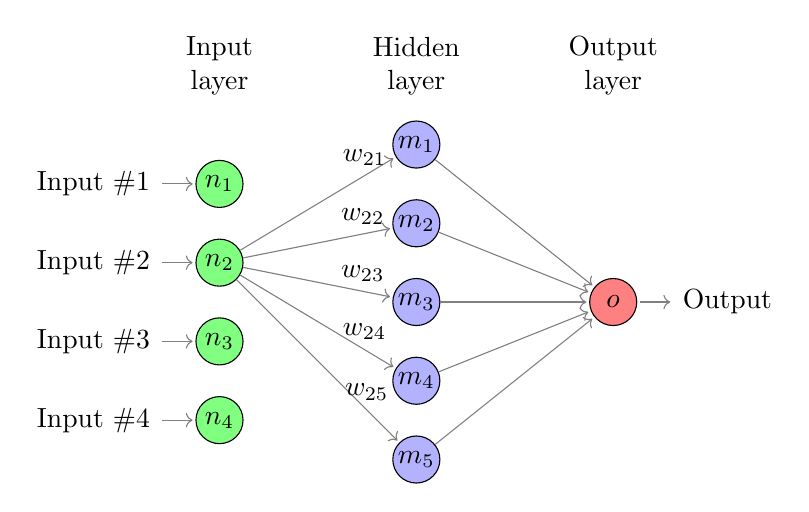
\begin{tikzpicture}[shorten >=1pt,->,draw=black!50, node distance=\layersep]
%https://tex.stackexchange.com/questions/96846/how-to-place-label-in-middle-of-line-above-and-below-with-tikz
    \tikzstyle{every pin edge}=[<-,shorten <=1pt]
    \tikzstyle{neuron}=[circle,fill=black!25,minimum size=17pt,inner sep=0pt, draw=black]
    \tikzstyle{input neuron}=[neuron, fill=green!50];
    \tikzstyle{output neuron}=[neuron, fill=red!50];
    \tikzstyle{hidden neuron}=[neuron, fill=blue!30];
    \tikzstyle{annot} = [text width=4em, text centered]

    % Draw the input layer nodes
    \foreach \name / \y in {1,...,4}
    % This is the same as writing \foreach \name / \y in {1/1,2/2,3/3,4/4}
        \node[input neuron, pin=left:Input \#\y] (I-\name) at (0,-\y) {$n_\y$};

    % Draw the hidden layer nodes
    \foreach \name / \y in {1,...,5}
        \path[yshift=0.5cm]
            node[hidden neuron] (H-\name) at (\layersep,-\y cm) {$m_\y$};

    % Draw the output layer node
    \node[output neuron,pin={[pin edge={->}]right:Output}, right of=H-3] (O) {$o$};

    % Connect every node in the input layer with every node in the
    % hidden layer.
%    \foreach \source in {1,...,4}
%        \foreach \dest in {1,...,5}
%            \draw (I-\source) -- node[below] {$w_ij$} ++ (H-\dest);


%    \foreach \source in {1,...,4}
        \foreach \dest in {1,...,5}
            \draw (I-2) -- node[above, pos=0.8] {$w_{2\dest}$} ++ (H-\dest);

    % Connect every node in the hidden layer with the output layer
    \foreach \source in {1,...,5}
        \path (H-\source) edge (O);

    % Annotate the layers
    \node[annot,above of=H-1, node distance=1cm] (hl) {Hidden layer};
    \node[annot,left of=hl] {Input layer};
    \node[annot,right of=hl] {Output layer};
\end{tikzpicture}
  \end{minipage}
  \vfill
\begin{minipage}[t][0.5\textheight][t]{\textwidth}

\end{minipage}


\end{frame}




\begin{frame}[fragile]{Point Variance of Linear Predictor}

\begin{align*}
\action<+->{ &=&&}
\\
\action<+->{  &=   && }
\end{align*}
\action<+->{The}
\end{frame}



\begin{frame}[fragile]{Correlation}
\begin{itemize}
\item[] \textbf{Serial No.} is basically uncorrelated with anything. \pause
\item[] \textbf{Admit} is highly correlated with \textbf{CGPA}, \textbf{TOEFL Score} and \textbf{GRE Score}\pause
\item[] \textbf{Research} has a lowish correlation with \textbf{Admit}, but also with everything else.  
\end{itemize}
\end{frame}











\begin{frame}[fragile]{Bias, Variance and Parameters}
  \begin{minipage}[t][0.5\textheight][t]{\textwidth}
	\centering
	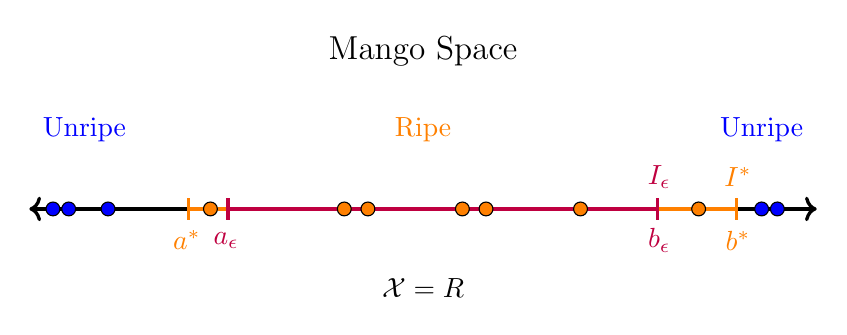
\begin{tikzpicture}
		\draw[<->,very thick] (-5,0) -- (5,0);
		\draw[color = orange, |-|,very thick] (-3,0) -- (4,0);
		\node[color=orange] at (4,.4) {$I^*$};
		\node at (0,2) {\large Mango Space} ;
		\node at (0,-1) {$\mathcal{X} = \mathbb{R}$} ;
		\node [color=blue] at (-4.3,1) {Unripe} ;
		\node [color=blue] at (4.3,1) {Unripe} ;
		\node [color=orange] at (0,1) {Ripe} ;

		\node [color=orange] at (-3,-.4) {$a^*$} ;
		\node [color=orange] at (4,-.4) {$b^*$} ;

		\draw [color=purple, |-|,very thick] (-2.5,0) -- (3,0);
		\node [color=purple] at (3,.4) {$I_\epsilon$} ;
		\node [color=purple] at (-2.5,-.4) {$a_\epsilon$} ;
		\node [color=purple] at (3,-.4) {$b_\epsilon$} ;

%		\draw [color=olive, |-|,very thick] (-3.5,0) -- (2.5,0);
%		\node [color=olive] at (3,.4) {$h_{\mathcal{T}}$} ;



		\node[circle,draw=black, fill=orange, inner sep=0pt,minimum size=5pt] at (2,0) {};
		\node[circle,draw=black, fill=orange, inner sep=0pt,minimum size=5pt] at (-1,0) {};
		\node[circle,draw=black, fill=orange, inner sep=0pt,minimum size=5pt] at (-.7,0) {};
		\node[circle,draw=black, fill=orange, inner sep=0pt,minimum size=5pt] at (.5,0) {};
		\node[circle,draw=black, fill=orange, inner sep=0pt,minimum size=5pt] at (.8,0) {};
		\node[circle,draw=black, fill=orange, inner sep=0pt,minimum size=5pt] at (-2.7,0) {};
		\node[circle,draw=black, fill=orange, inner sep=0pt,minimum size=5pt] at (3.5,0) {};

		\node[circle,draw=black, fill=blue, inner sep=0pt,minimum size=5pt] at (-4.5,0) {};
		\node[circle,draw=black, fill=blue, inner sep=0pt,minimum size=5pt] at (-4,0) {};
		\node[circle,draw=black, fill=blue, inner sep=0pt,minimum size=5pt] at (-4.7,0) {};
		\node[circle,draw=black, fill=blue, inner sep=0pt,minimum size=5pt] at (4.3,0) {};
		\node[circle,draw=black, fill=blue, inner sep=0pt,minimum size=5pt] at (4.5,0) {};
	\end{tikzpicture}
  \end{minipage}
  \vfill
  \begin{minipage}[t][0.5\textheight][t]{\textwidth}
Lets understand this visually.
$$
Err(x_0) = \sigma_\epsilon^2 + [E_\cT[\hat f(x_0)] - f(x_0)]^2 + E_\cT\big[ \hat{f}(x_0) - E_\cT[\hat{f}(x_0)] \big]^2\,.
$$\pause
Consider a data set, 
\end{minipage}
\end{frame}





























